%%%%%%%%%%%%%%%%%%%%%%%%%%%%%%%%%%%%%%%%%%%%%%%%%%%%%%%%%%%%%%%%%%%%%%%%
% Copyright (c) 2022 Antonio Coín Castro
%
% This work is licensed under a
% Creative Commons Attribution-ShareAlike 4.0 International License.
%
% You should have received a copy of the license along with this
% work. If not, see <http://creativecommons.org/licenses/by-sa/4.0/>.
%%%%%%%%%%%%%%%%%%%%%%%%%%%%%%%%%%%%%%%%%%%%%%%%%%%%%%%%%%%%%%%%%%%%%%%%

\let\epsilon\varepsilon

%%%%%%%%%%%%%%%%%%%%%%%%%%%%%%%%%%%%%%%%%%%%%%%%%%%%%%%%%%%%%%%%%%%%%%%%
\chapter{Background and related work}\label{ch:background}
%%%%%%%%%%%%%%%%%%%%%%%%%%%%%%%%%%%%%%%%%%%%%%%%%%%%%%%%%%%%%%%%%%%%%%%%

FDA is undoubtedly an active area of research, which finds applications in a wide variety of fields, such as biomedicine, finance, meteorology or chemistry \citep[see for example][]{ullah2013applications}. Accordingly, there are many recent contributions on how to tackle functional data problems, both from a theoretical and practical standpoint. Chief among them is the approach of reducing the problem to a finite-dimensional one, for example using a truncated basis expansion or spline interpolation methods \citep[e.g.][]{muller2005generalized, aguilera2013comparative}. At the same time, much effort has also been put into the task of building a sound theoretical basis for FDA, generalizing different concepts to the infinite-dimensional framework. Examples of this endeavor include the definition of centraility measures and depth-based notions for functional data \citep[e.g.][]{fraiman2001trimmed, cuevas2007robust, lopez2009concept}, an ANOVA test for functional data \citep{cuevas2004anova}, a purely functional partial least squares algorithm \citep{delaigle2012methodology}, a functional Mahalanobis distance \citep{berrendero2020mahalanobis}, or an extension of Fisher's discriminant analysis for function-valued random elements \citep[e.g.][]{james2001functional, shin2008extension}, among many others. Interestingly enough, these last two are examples of situations in which a RKHS-based approach provides useful insights.

Another technique found in the related literature is the use of Gaussian processes to model the functional behavior of the data \citep[see for instance][]{shi2011gaussian}. These ideas extend the theory of Gaussian process regression in classical finite-dimensional settings \citep[e.g.][]{rasmussen2004gaussian}, providing an alternative Bayesian approach to functional inference and prediction problems. Additional non-parametric methods for functional prediction and classification were notably explored in \citet{ferraty2006nonparametric}.

\subsection*{\(L^2\)-models}

 The most common scalar-on-function linear regression model is the classical \(L^2\)-model, widely popularized since the first edition (1997) of the monograph by~\citet{ramsay2005functional}. It can be seen as a generalization of the usual finite-dimensional model, replacing the scalar product in \(\R^p\) for that of the functional space \(L^2[0,1]\):
\begin{equation}\label{eq:l2-linear-model}
Y = \alpha_0 + \dotprod{X}{\beta} + \epsilon = \alpha_0 + \int_0^1 X(t)\beta(t)\, dt + \epsilon,
\end{equation}
where \(\alpha_0\in \R\), \(\epsilon\) is a random error term independent from \(X\) with \(\E [\epsilon]=0\), and the functional slope parameter \(\beta=\beta(\cdot)\) is assumed to be a member of the infinite-dimensional space \(L^2[0, 1]\). A careful rearrangement of~\eqref{eq:l2-linear-model} shows that the model is equivalently expressed as \(\Delta=\K\beta\), where \(\Delta(\cdot)\) is the cross-covariance function of \(X\) and \(Y\), and \(\K\) is the covariance operator of the process \(X\) (to be defined in Section~\ref{sec:rkhs}). This expression is a continuous analog of the normal equations that arise in finite-dimensional regression settings, and since the operator \(\K\) is non-invertible in general, questions of existence and unicity of \(\beta\) need further study \citep[see][]{cardot2011functional}.

Technical details aside, the inference on \(\beta\) is also hampered by the fact that \(L^2[0,1]\) is an extremely wide space that contains many non-smooth or ill-behaved functions, so that any estimation procedure involving optimization on it would typically be hard.
Although it can be tempting to simply discretize the observed values on a grid and proceed with standard multiple linear regression, this would result in an under-determined model in which the estimated parameters lose meaning. This happens essentially because the number of available parameters is infinite, but the number of equations is finite \citep[see][Sec.~15.2]{ramsay2005functional}. Thus, some regularization or dimensionality reduction techniques are needed for parameter estimation; see \citet{reiss2017methods} for a summary of several widespread methods.

A common inference strategy is to expand both \(X\) and \(\beta\) on a certain data-driven orthonormal basis of \(L^2[0,1]\), say \(\{\phi_j\}\), up to a certain value \(p\in\N\):

\[
  X(t)=\sum_{j=1}^p Z_j \phi_j(t), \quad \beta(t) = \sum_{j=1}^p \beta_j \phi_j(t).
\]
In this way, model~\eqref{eq:l2-linear-model} simplifies to
\[
Y = \alpha_0 + \sum_{j=1}^p \beta_j Z_j,
\]
which can then be solved in the usual manner. For example, when the chosen basis is composed of eigenfunctions of the covariance operator \(\K\), this method is known as Functional Principal Component Regression (FPCR). Another class of methods focus on selecting an \textit{a priori} basis for \(\beta\) (e.g. a spline basis) and solving a penalized least squares problem. In particular, for a truncated basis representation of the form \(\beta(t)=\phi(t)'b\), with \(\phi(t)=(\phi_1(t), \dots, \phi_p(t))'\) and \(b\in\R^p\), a typical minimization problem would be
\[
\argmin_{(\alpha_0, b)\in\R\times\R^p} \ \left\{ \sum_{i=1}^n \left( y_i - \alpha_0 - \int_0^1 x_i(t)[\phi(t)'b]\, dt\right)^2 + \lambda \Omega(b) \right\},
\]
where \(\Omega\) is some penalty function and \(\lambda>0\) is a regularization parameter.

Turning our attention to logistic regression, a similar \(L^2\)-based functional logistic equation can be derived for the binary classification problem via the logistic function:
\begin{equation}\label{eq:l2-logistic-model}
  \P(Y=1 \mid X) = \frac{1}{1 + \exp\{-\alpha_0 - \dotprod{X}{\beta}\}},
\end{equation}
where \(\alpha_0 \in \R\) and \(\beta \in L^2[0, 1]\). In this situation, the most common way of estimating the slope function \(\beta\) is via its Maximum Likelihood Estimator (MLE). However, not only do the same complications as in the linear regression model apply in this situation, but there is also the additional problem that in functional settings the MLE does not exist with probability one under fairly general conditions \citep[see][Sec.~3.2]{berrendero2018functional}.

\subsection*{RKHS models}

In spite of the apparent generality of model~\eqref{eq:l2-linear-model}, it can be shown that it is not flexible enough to include ``simple'' finite-dimensional models based on linear combinations of the marginals, such as \(Y=\alpha_0 + \beta_1 X(t_1)+ \cdots + \beta_p X(t_p) + \epsilon\) for some constants \(\beta_j\in\R\) and instants \(t_j\in[0,1]\); see \citet{berrendero2020general} for additional details on this. It turns out that in both linear and logistic scenarios a natural alternative to the \(L^2\)-model is the so-called Reproducing Kernel Hilbert Space (RKHS) model, which instead assumes the unknown functional parameter to be a member of the RKHS associated with the covariance function of the process \(X\), making use of the scalar product of that functional space. As we will show later on, not only is this model simpler and arguably easier to interpret, but it also constrains the parameter space to smoother and more manageable functions. In fact, it does include a model based on finite linear combinations of the marginals of \(X\) as a particular case, which is especially appealing to practitioners confronted with functional data problems due to its simplicity. These RKHS-based models and their idiosyncrasies have been explored in \citet{berrendero2019rkhs, berrendero2020general} in the functional linear regression setting, and in \citet{berrendero2018functional} for the case of functional logistic regression.

There are other proposals for models that change the habitat of the functional parameter, and there are even some in which \(\beta\) is supposed to live in a RKHS, most notably \citet{yuan2010reproducing}. However, theirs are arbitrary RKHS's that do not directly exploit the relation with the process \(X\) (though the authors do use this connection to derive some asymptotic properties of their estimators), and therefore the approach is somewhat different. Incidentally, the RKHS associated with \(X\) also has some interesting properties that contribute to shed light on the near-perfect classification phenomenon for functional data, described by \citet{delaigle2012achieving} and further examined for example in the works of \citet{berrendero2018use} or \citet{torrecilla2020optimal}.

A major aim of this work is to motivate these recently-proposed RKHS models inside the functional framework, while also providing efficient techniques to apply them in practice. Our main contribution is the proposal of a Bayesian approach to parameter estimation within the aforementioned RKHS models, in which a prior distribution is imposed on the unknown functional parameter to obtain a posterior distribution after seeing the data. Although setting a prior distribution on a functional space is generally a hard task, the specific parametric formulation of the RKHS models we propose greatly facilitates this (see Chapter~\ref{ch:bayesian} for details). A similar Bayesian scheme has recently been explored in \citet{grollemund2019bayesian}, albeit not within a RKHS framework.

Another set of techniques extensively studied in this context are variable selection methods, which aim to select the marginals \(\{X(t_j)\}\) of the process that better summarize it according to some optimality criterion. As it happens, some variable selection methods have already been proposed in the RKHS framework \citep[see for example][]{berrendero2019rkhs}, but in general they have their own dedicated algorithms and procedures. As will become apparent in the forthcoming chapters, given the nature of our suggested Bayesian model we can easily isolate the marginal posterior distribution corresponding to a finite set of points \(\{t_j\}\), and thus provide a Bayesian-motivated variable selection process along with the other prediction methods that naturally arise within our model. In this way, in addition to making predictions about the input data, we can evaluate exactly which marginals of the functional explanatory variable contain the most relevant information. These points-of-impact selection models for functional predictors have also been considered in the  literature; see \citet{poss2020superconsistent}, \citet{berrendero2016variable} or \citet{ferraty2010most} by way of illustration. Another example of a related strategy is the work of \citet{james2009functional}, in which the authors propose a method to estimate \(\beta(t)\) in such a way that it is exactly zero over some regions in the domain (a sort of ``region selection'' algorithm).


\subsection*{Bayesian inference}

The term Bayesian inference usually refers to a wide class of methods that to some extent employ Bayes' theorem to update the initial probability assigned to a hypothesis (or a parameter) when new information is available. It can be seen as a general tool for modeling situations or problems that involve uncertainty; some examples include Bayesian hierarchical modeling, Bayesian regression or even Bayesian neural networks \citep[see e.g.][]{murphy2012machine, bishop2006pattern}. Specifically, in this work we will be interested in performing parameter estimation in a Bayesian framework, so that pre-existing information and beliefs about the parameters can be incorporated into the model.

One difficulty found in almost all Bayesian methods is that the posterior distribution, the main object of interest, is usually intractable due to the integral that appears as the normalizing constant in Bayes' rule. A way to bypass this limitation is to use conjugate distributions, where it can be rigorously proven that a certain combination of likelihood and prior distributions produces a posterior distribution in the same family as the prior. However, unless conjugate priors are used, a closed-form expression is generally unattainable and some type of approximation is required. Apart from basic numerical integration, some well-performing methods in this regard are variational inference approaches \citep[e.g.][]{blei2017variational} and MCMC methods \citep[e.g.][]{brooks2011handbook}. The former are based on approximating the posterior by another distribution restricted to a certain parametric family so that the Kullback-Leibler divergence between them is minimized, whereas the latter are iterative methods that directly provide approximate samples of the posterior distribution.

On a separate note, there are some recent works that tackle Bayesian inference from a functional perspective, mostly in relation to the distribution over functions induced by Bayesian neural networks. Some examples are the functional Bayesian neural networks proposed by~\citet{sun2019functional}, variational implicit processes \citep{ma2019variational} and their deep variants \citep{ortega2022deep}, or the functional variational inference approach suggested in~\citet{ma2021functional}. Moreover, there are approaches to functional regression from a Bayesian perspective that impose a Gaussian process prior on the functional parameter \(\beta\) \citep[e.g][]{lian2016posterior}, and it turns out that the RKHS's corresponding to these Gaussian processes, described for example in~\citet{van2008reproducing}, are useful when studying contraction rates of the posterior distribution.

\section{Reproducing kernel Hilbert spaces}\label{sec:rkhs}

In this section we present a brief exposition of some basic concepts regarding reproducing kernel Hilbert spaces. Although there are quite a few ways of introducing these spaces, we adopt a probabilistic point of view that will set the stage for the development of the subsequent theory. For a more detailed account, a good reference is the book by~\citet{berlinet2004reproducing}. Although the following ideas can be extended to complex functions, we restrict ourselves to real-valued functions for the sake of simplicity. We start by defining the concept of kernel functions, which are the foundation of these spaces.

\begin{definition}
  We say that a function of two variables \(K: \T \times \T \to \R\) is positive semidefinite\footnote{Sometimes in the literature these functions are known simply as positive definite.} if
  \[
    \sum_{i,j=1}^p a_ia_jK(t_i, t_j) \geq 0
  \]
  for any \(p\in\N\), any \((a_1,\dots, a_p)\in \R^p\) and any \((t_1,\dots, t_p)\in\T^p\). Note that this is equivalent to saying that the matrix \((K(t_i, t_j))_{i,j}\) is positive semidefinite for any choice of \(p\in\N\) and \((t_1,\dots, t_p)\in\T^p\).
\end{definition}

We will be interested mainly in positive semidefinite functions that are symmetric, which are usually referred to as \textit{kernel functions}, and which happen to be the class of covariance functions of second order stochastic processes \citep[][Th. 27]{berlinet2004reproducing}. Let us now show how a RKHS arises from a kernel function.

Suppose \(X=X(t)\) is a \(L^2\)-stochastic process with trajectories in \(L^2[0, 1]\), and for simplicity assume \(\E[X(t)]=0\) for all \(t\in[0,1]\). Let us denote by \(K(t, s)= \E[X(t)X(s)]\) the covariance function of the process \(X\). To construct the RKHS \(\Hcal(K)\) associated with the covariance function, we start by defining the functional vector space \(\Hcal_0(K)\) of all finite linear combinations of evaluations of \(K\), that is,
\begin{equation}\label{eq:h0}
\Hcal_0(K) = \left\{ f: \ f(\cdot) = \sum_{i=1}^p a_i K(t_i, \cdot), \ p \in \N, \ a_i \in \R, \ t_i \in [0, 1] \right\}.
\end{equation}
Note that, as subsets, \(\Hcal_0(K)\subset L^2[0,1]\). However, this new space can be endowed with an inner product different from the one induced by \(L^2[0,1]\), namely
\[
\dotprod{f}{g}_K = \sum_{i, j} a_i b_j K(t_i, s_j),
\]
for \(f(\cdot)=\sum_i a_i K(t_i, \cdot) \) and \(g(\cdot)=\sum_j b_j K(s_j, \cdot)\). We show below that it is well defined, but before we note that functions in this space satisfy the so-called \textit{reproducing property}: \(f(t) = \dotprod{K(t, \cdot)}{f}_K\) for all \(t \in [0, 1]\). In particular, \(K(t, s)=\dotprod{K(t, \cdot)}{K(s, \cdot)}_K\), which can be understood as saying that the kernel \textit{reproduces} itself, hence the term ``reproducing kernel''.

\begin{proposition} \((\Hcal_0(K), \dotprod{\cdot}{\cdot}_K)\) is an inner product space.
\end{proposition}
  \begin{proof}
    Firstly, consider \(f(\cdot)=\sum_i a_i K(t_i, \cdot) \) and \(g(\cdot)=\sum_j b_j K(s_j, \cdot)\), and observe that
    \[
      \dotprod{f}{g}_K = \sum_j b_j f(s_j) = \sum_i a_i g(t_i).
    \]
    These equalities show that \(\dotprod{f}{g}_K\) depends only on \(f\) and \(g\) through their values, so it is independent of their representation in \(\Hcal_0(K)\). From this expression (and also from the original definition) it is straightforward to check linearity and symmetry, while positive semidefiniteness is a direct consequence of \(K\) being a covariance function, and thus positive semidefinite. It remains to prove that \(\dotprod{f}{f}_K=0\) implies \(f=0\). Indeed, for all \(t\in[0,1]\) and \(\epsilon \in \R\), we have
    \[
    0 \leq \dotprod{f + \epsilon K(t, \cdot)}{f + \epsilon K(t, \cdot)}_K = \dotprod{f}{f}_K + 2\epsilon\dotprod{f}{K(t, \cdot)}_K + \epsilon^2 K(t, t).
    \]
    Now, if \(\dotprod{f}{f}_K=0\), by letting \(\epsilon\to 0^{\pm}\) we see that \(f(t)=\dotprod{f}{K(t, \cdot)}_K\) necessarily vanishes for all \(t\), as desired.
  \end{proof}

At this point, \(\Hcal(K)\) is defined to be the completion of \(\Hcal_0(K)\) under the norm induced by the scalar product \(\dotprod{\cdot}{\cdot}_K\), which informally amounts to adding all the limits of Cauchy sequences in \(\Hcal_0(K)\), turning it into a genuine Hilbert space with the inner product extended accordingly. Then it is immediate to see that the reproducing property is retained. An important consequence is that \(\Hcal(K)\) is a space of actual functions and not of equivalence classes, since the values of the functions at particular points are in fact relevant, unlike in \(L^2\)-spaces.

Indeed, another way of defining a RKHS is via the continuity of all the \textit{evaluation operators}, i.e., \(\delta_t(f) := f(t)\) for \(f\in\Hcal(K)\) and \(t\in[0,1]\). In this case, the interpretation is that if two functions are close in the RKHS norm, they are also pointwise close. Although in this definition there is no explicit mention of the kernel, it can be recovered through the Riesz representation theorem. We summarize below some interesting topological properties of \(\Hcal(K)\).

\begin{proposition} The following properties hold for the space \(\Hcal(K)\):
  \begin{enumerate}
    \item The evaluation operator \(\delta_t\) is bounded for all \(t\in[0,1]\).
    \item Norm convergence implies pointwise convergence, and if \(K\) is continuous, it also implies uniform convergence.
    \item If \(K\) is m-times continuously differentiable, then so is every function \(f\in\Hcal(K)\). In particular, if \(K\) is continuous, every function \(f\in\Hcal(K)\) is continuous.
  \end{enumerate}
\end{proposition}
\begin{proof}
  To prove \((i)\), simply note that for any \(t\in[0,1]\) and \(f\in\Hcal(K)\) the Cauchy-Schwarz inequality and the reproducing property tell us that
  \[
  |\delta_t(f)| = |f(t)| = |\dotprod{f}{K(t, \cdot)}_K| \leq \|K(t, \cdot)\|_K \|f\|_K = \sqrt{K(t, t)}\|f\|_K,
  \]
  and consequently \(\|\delta_t\|\leq \sqrt{K(t, t)}\). To see \((ii)\), observe that for any \(t\in[0,1]\) we have
  \[
    |f_n(t) - f(t)| = |\delta_t(f_n - f)| \leq \|\delta_t\|\|f_n - f\|_K,
  \]
  as we have just shown in \((i)\) that the evaluation operator is bounded. Moreover, if \(K\) is continuous on its (compact) domain, \(\|\delta_t\| \leq \sup_s \sqrt{K(s, s)}=M<\infty\) for all \(t\), so the convergence is indeed uniform. Finally, we prove the second statement in \((iii)\), and refer the reader to \citet[][Th 2.6]{saitoh2016theory} for a complete proof. If \(K\) is continuous, then it is clear that every function in \(\Hcal_0(K)\) is continuous. Let us now fix an arbitrary \(f\in \Hcal(K)\). By definition, there exists a sequence \(\{f_n\}\subset \Hcal_0(K)\) of continuous functions such that \(\|f_n - f\|_K \to 0\). But then \(f_n \to f\) uniformly by \((ii)\), and therefore \(f\) is continuous as the uniform limit of continuous functions. Note that this statement remains valid, with a slightly different proof, even when the underlying domain is not compact.
\end{proof}

For the sake of completeness, it is worth mentioning that the RKHS associated with a kernel function is unique, and indeed the Moore-Aronszajn theorem \citep[e.g.][Th. 3]{berlinet2004reproducing} states that there is a one-to-one correspondence between kernel functions and reproducing kernel Hilbert spaces. Let us now illustrate the definition in a few simple cases; see \citet[][Ch.~1]{saitoh2016theory} for more involved examples.

\begin{example}\label{ex:bm}
  If \(X\) is the standard Brownian motion on \([0, 1]\), it is well known that the associated covariance function is \(K_{\text{bm}}(t, s) = \min\{t,s\}\). The corresponding RKHS is given by \citep[][Ex. 8.19]{janson1997gaussian}:
  \[
    \Hcal(K_{\text{bm}}) = \{f: f \text{ is absolutely continuous, } f(0)=0 \text{ and } f'\in L^2[0, 1]\},
  \]
  with inner product \(\dotprod{f}{g}_{K_{\text{bm}}} = \int f'g'\).
\end{example}

\begin{example}[Finite-dimensional RKHS]
  Setting aside our stochastic process framework for a moment, we can conceive examples outside of \(\T =[0,1]\). Consider a vector-valued random variable \(X = (X_1, \dots, X_p)\) with non-singular covariance matrix \(\Sigma\). In this case the index set would be \(\T_p = \{1,\dots,p\}\), so identifying functions on \(\T_p\) with points in the \(p\)-dimensional Euclidean space, we have \(\Hcal(\Sigma)=\R^p\), with inner product \(\dotprod{x}{y}_\Sigma=x\Sigma^{-1}y\).
\end{example}

\begin{example}[Non-RKHS Hilbert space]
  As we pointed out before, the space of square integrable functions \(L^2(\R)\) \textit{is not} a RKHS. There are many ways of seeing this; for example, in this space norm convergence does not imply pointwise convergence. Another possibility is to observe that the would-be reproducing kernel must be the Dirac delta function:
  \[
    f(s) = \int_{-\infty}^\infty f(t)\delta(t, s)\, dt \quad \forall s \in \R.
  \]
  However, \(\delta(t, \cdot) \notin L^2(\R)\).
\end{example}

\subsection*{The covariance operator}

 Note that, as expected, the covariance function of \(X\) plays a crucial role in characterizing the associated RKHS. An integral operator closely related to the kernel is the so-called covariance operator, namely
\[
\K f(\cdot) = \int_0^1 K(s, \cdot)f(s)\, ds, \quad f \in L^2[0, 1],
\]
which is self-adjoint and compact when \(K\) is continuous \citep[e.g.][Th.~4.6.2]{hsing2015theoretical}, so for the remaining of this work we will indeed suppose that \(K\) is continuous. As it turns out, the covariance function admits a spectral decomposition in terms of the eigenvalues and eigenfunctions of this integral operator, a sort of continuous generalization of the eigendecomposition of a symmetric positive semidefinite matrix.

\begin{theorem}[Mercer's theorem]\label{th:mercer}
    Let \(K\) be a continuous kernel on \([0,1]^2\). Then, there exists an orthonormal system \(\{\phi_j\}\) in \(L^2[0,1]\) consisting of eigenfunctions of \(\K\), whose corresponding eigenvalues are all positive and form a non-increasing sequence \(\{\lambda_j\}\to 0\), and such that
    \[
      K(t, s) = \sum_{j=1}^\infty \lambda_j \phi_j(t)\phi_j(s)
    \]
    for all \(t\) and \(s\), where the convergence is absolute and uniform.
\end{theorem}

In connection with our RKHS theory, it can be shown that the set \(\{\sqrt{\lambda_j}\phi_j\}\) constitutes an orthonormal basis of \(\Hcal(K)\) \citep[see e.g.][Sec.~4.4]{cucker2007learning}. Furthermore, a similar orthogonal decomposition holds for our stochastic process \(X\), an expansion which lies at the base of many \(L^2\) functional regression models. The proof of the following result, along with the proof of Mercer's theorem, can be consulted in \citet[][Sec.~3.2]{berlinet2004reproducing}.

\begin{theorem}[Karhunen-Loève expansion]
  With the assumptions and notations of Theorem~\ref{th:mercer}, the centered process \(X=X(t)\) with covariance function \(K\) admits the quadratic-mean representation
  \[
  X(t) = \sum_{j=1}^\infty \zeta_j \phi_j(t),
  \]
  where the convergence is in \(L^2(\Omega)\) and uniform in \(t\). The \(\zeta_j\) are independent zero-mean random variables with \(\E[\zeta_i\zeta_j]=\delta_{ij}\lambda_j\), given explicitly by the formula
  \[
    \zeta_j = \int_0^1 X(t)\phi_j(t)\, dt, \quad j\geq 1.
  \]
\end{theorem}

In addition to these results, it is worth mentioning that the covariance operator \(\K\) provides several alternative definitions of \(\Hcal(K)\). For example, the RKHS can be identified with the image of the operator's square root, i.e., \(\Hcal(K) = \K^{1/2}(L^2[0, 1])\), with inner product \(\dotprod{f}{g}_K = \dotprod{\K^{-1/2}(f)}{\K^{-1/2}(g)}\). Furthermore, we can think of the norm in \(\Hcal(K)\) as an \(L^2\)-like regularized norm, since this space can also be seen as the set \(\Hcal(K) = \{f \in L^2[0, 1]: \ \sum_j \lambda_j^{-1}\dotprod{f}{\phi_j}^2 < \infty \}\), with corresponding inner product \(\dotprod{f}{g}_K = \sum_j \lambda_j^{-1}\dotprod{f}{\phi_j}\dotprod{g}{\phi_j}\). Note that, since \(\{\lambda_j\}\) tends to zero, this definition highlights the fact that functions in \(\Hcal(K)\) are smooth, not only in that they inherit the regularity of the kernel \(K\), but also in the sense that their components in an orthonormal basis, namely \(\dotprod{f}{\phi_j}\), need to vanish quickly.

\subsection*{Loève's isometry}

Until now we have seen that \(\Hcal(K)\) is a space related to \(X\) only through its covariance function. Nevertheless, we will now hopefully clarify that this space can indeed be seen as \textit{the} Hilbert space inherently associated with the process \(X\) itself. Let us shift the perspective momentarily and consider the linear span of \(X\) in the space of all zero-mean random variables with finite second moment, i.e.:
\[
\Lcal_0(X) = \left\{\sum_{i=1}^p a_i X(t_i): p\in\N, \ a_i \in \R, \ t_i \in [0,1]\right\}.
\]
It is well known that its completion in \(L^2(\Omega)\), denoted \(\Lcal(X)\), is a Hilbert space, sometimes called the Hilbert space generated by \(X\). In the words of \citet{berlinet2004reproducing}, ``\(\Lcal(X)\) \textit{contains the random variables attainable by linear operations, including limits, on the measurements of the process}''. As it happens, via \textit{Loève's isometry} \citep{loeve1948fonctions} one can establish a congruence \(\Psi_X\) between \(\Hcal(K)\) and \(\Lcal(X)\) \citep[see Lemma 1.1 in][]{lukic2001stochastic}. This isometry is essentially the completion of the correspondence
  \begin{equation}\label{eq:loeves-isometry}
  \sum_{i=1}^p a_i X(t_i) \longleftrightarrow \sum_{i=1}^p a_i K(t_i, \cdot),
  \end{equation}
and can be formally defined, in terms of its inverse, as \(\Psi^{-1}_X(U)(t) = \E[U X(t)]\) for \(U \in \Lcal(X)\). Thus, \(\Hcal(K)\) can be regarded as an isometric copy of \(\Lcal(X)\), an approach that is often useful in statistics.

However, despite the close connection between the process \(X\) and the space \(\Hcal(K)\), special care must be taken when dealing with concrete realizations of the process. It can be shown that under rather general conditions the trajectories of \(X\) \textit{do not belong} to the corresponding RKHS with probability one \citep[see for example][Cor.~7.1]{lukic2001stochastic}. For instance, the trajectories of a Brownian motion are known to be nowhere differentiable, but as shown in Example~\ref{ex:bm}, the elements of the corresponding RKHS are differentiable almost everywhere. An heuristic argument to justify this fact, given in \citet{wahba1990spline}, is as follows: consider the Karhunen-Loève expansion of \(X\), i.e.,
\[
  X(t) = \sum_{j=1}^\infty \zeta_j \phi_j(t),
\]
and the truncated version \(X_N(t)\) up to the \(N\)-th term. On the one hand, for each fixed \(t\) we have \(X_N(t)\to X(t)\) in the quadratic mean sense (by the Karhunen-Loève theorem), but on the other hand observe that
\[
  \E\left[\|X_N(\cdot)\|^2_K\right] = \E \left[\sum_{j=1}^N \frac{\zeta_j^2}{\lambda_j}\right] = N \to \infty \quad (N\to\infty).
\]

As a consequence, the expression \(\dotprod{x}{f}_K\) is ill-defined and lacks meaning when \(x\) is a realization of \(X\). However, following Parzen's approach in his seminal work \citep[e.g.][Th.~4E]{parzen1961approach}, we can leverage Loève's isometry and identify \(\dotprod{x}{f}_K \) with the image \( \Psi_x(f) := \Psi_X(f)(\omega)\), for \(x=X(\omega)\) and \(f\in \Hcal(K)\). This notation, viewed as a formal extension of the inner product, often proves to be useful and convenient. Some properties stemming from this interpretation are stated below \citep[see][p.~974]{parzen1961approach}.

\begin{proposition}
  For every \(t\in[0,1]\) and \(f, g \in \Hcal(K)\), the following relations are satisfied:
\begin{enumerate}
  \item \(\dotprod{X}{K(t, \cdot)}_K = X(t)\), a particular reproducing property.
  \item \(\E[\dotprod{X}{f}_K] = 0\).
  \item \(\E[\dotprod{X}{f}_K\dotprod{X}{g}_K] = \dotprod{f}{g}_K\).
\end{enumerate}
\end{proposition}
Note that the statement \((iii)\) above provides yet another characterization of the inner product in \(\Hcal(K)\), where \(\dotprod{X}{f}_K\) and \(\dotprod{X}{g}_K\) are understood as the random variables representing \(f\) and \(g\) in \(\Lcal(X)\), respectively.


\subsection*{Applications in machine learning}

Although not the main concern of this work, the theory of reproducing kernels and the associated kernel methods find applications in many areas of machine learning. For example, the well-known \textit{kernel trick} can be seen as a specific application of the reproducing property, where a feature map \(\Phi(x) \in \Hcal\) is applied to the objects in the space of interest, transforming them into richer elements in a RKHS. Then, many computations can be efficiently carried out in an implicit manner by means of the corresponding kernel
\[
K(x, y)=\dotprod{\Phi(x)}{\Phi(y)}_{\Hcal}.
\]
The fact that one does not need to explicitly compute \(\Phi(x)\) is especially relevant for kernels with a simple expression but a possibly complex feature space (e.g. infinite-dimensional), such as the Gaussian kernel \(K(x, y)=\exp(-\gamma\|x-y\|^2)\).

Another example of the use of RKHS's is in the context of regularization problems, where the celebrated \textit{representer theorems} provide a way of obtaining closed-form solutions to a penalized optimization problem. For instance, learning techniques that rely on empirical risk minimization \citep[e.g.][]{vapnik1991principles} benefit from one such result by \citet{scholkopf2001generalized}, stated below.

\begin{theorem}[Generalized representer theorem]
  Consider a RKHS of functions \(\Hcal(K)\) defined over a non-empty set \(\X\), a training set \(\{(x_i, y_i)\}_{i=1}^n \subset (\X \times \R)^n\), an arbitrary error function \(R: (\X  \times \R^2)^n \to \R\cup\{\infty\}\), and a strictly increasing real-valued function \(\Omega:[0,\infty)\to \R\). Then, any minimizer \(f^\ast\) of the regularized empirical risk
  \[
    R(\{(x_i, y_i, f(x_i))\}_{i=1}^n) + \Omega(\|f\|_K)
  \]
  is of the form \(f^\ast(\cdot) = \sum_{i=1}^n a_i K(x_i, \cdot)\), where \(a_i\in\R\) for all \(i=1,\dots,n\).
\end{theorem}

\section{Markov chain Monte Carlo}\label{sec:mcmc}

In the context of Bayesian inference, there are many situations in which we would like to sample from a distribution without using its explicit closed-form density, either because we do not know it, or because it is computationally difficult to do so. In these cases, we could work with a function \(f(x)\) proportional to our target density \(\pi(x)\). More specifically, in a Bayesian framework the posterior distribution is often intractable due to the normalizing integral constant, but we do know that \(posterior \propto prior \times likelihood\).

When \(x\in\R\), we can use Monte Carlo algorithms such as \textit{rejection sampling}. In a nutshell, this method samples uniformly from the area under \(f(x)\) by means of an auxiliary density that encompasses this area. Specifically, one needs to find a density function \(g\) with \(\supp f \subset \supp g\) and \(f \leq Mg\) for some \(M>1\). Then, sampling from \(g\) and accepting the proposal, say \(x\), with probability \(f(x)/Mg(x)\) yields an approximate set of samples from \(f\). Nevertheless, these kinds of algorithms are rapidly affected by the so-called \textit{curse of dimensionality} (see the schematic in Figure~\ref{fig:curse_dimensionality}), so new techniques are needed when sampling from multidimensional distributions. This is where Markov chain Monte Carlo (MCMC) methods come into play.

\begin{figure}[ht!]
  \centering
  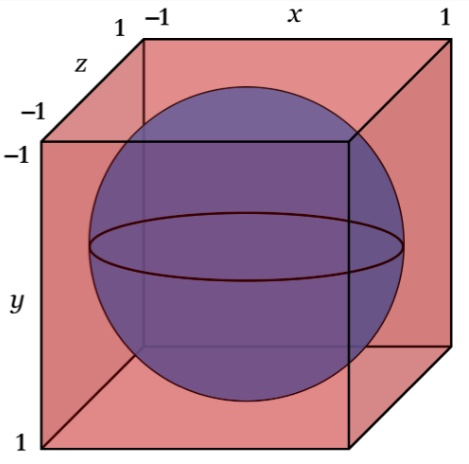
\includegraphics[width=.25\textwidth]{cube_sphere}
  \caption{To cover the volume of \(f(x)\) in higher dimensions we intuitively need a volume that grows exponentially with the dimension itself.}\label{fig:curse_dimensionality}
\end{figure}

MCMC methods are based on the iterative construction of a Markov chain whose stationary distribution is the objective distribution \(\pi(x)\). In this way, we can take the samples of a sufficiently advanced chain as approximate realizations of \(X\sim \pi(x)\). When it comes to building the chains, transition probabilities are assigned in such a way that regions with higher density with respect to \(\pi(x)\) are favored (by means of the known proportional function \(f(x)\)). The dimensionality issues are somewhat mitigated, and on top of that there are specific tuning techniques to tackle them. However, the samples obtained from this procedure are not independent, though they can be made so by \textit{thinning} the chain and considering only one every few samples.

Another advantage of these methods is that they recover the marginal distributions directly. Suppose that after a successful MCMC run we have \(M\) multivariate samples \(\{\theta^{(m)}=(\theta_1^{(m)},\dots, \theta_p^{(m)})\}\) of a joint \(p\)-dimensional distribution. The marginal distribution of each variable, which would be theoretically computed as
\[
\pi(\theta_i) = \int \pi(\theta)\,d\theta_1\,\cdots\,d\theta_{i-1}\,d\theta_{i+1}\,\cdots \,d\theta_p,
\]
can be approximated by just retaining the samples \(\{\theta_i^{(m)}\}\) corresponding to \(\theta_i\).

\subsection*{Metropolis-Hastings}

The Metropolis-Hastings algorithm \citep{metropolis1953equation} is arguably the best known algorithm in this context. As a matter of fact, it is actually more of a general framework from which many other methods are derived. In its original formulation, it relies on a symmetric \textit{proposal} distribution \(g(x'|x_t)\) that generates a proposal for the next state given the current one (e.g. a Gaussian distribution centered on \(x_t\)). Approximate samples from the intended distribution can then be generated through the following iterative acceptance-based procedure:
\begin{enumerate}[1.]
  \item Generate a proposal \(x' \sim g(x'|x_t)\).
  \item Accept the proposal with probability \(\alpha=\min\{1, f(x')/f(x_t)\}\). If accepted, set \(x_{t+1}=x'\); otherwise set \(x_{t+1}=x_t\).
\end{enumerate}

 \begin{figure}[ht!]
   \centering
   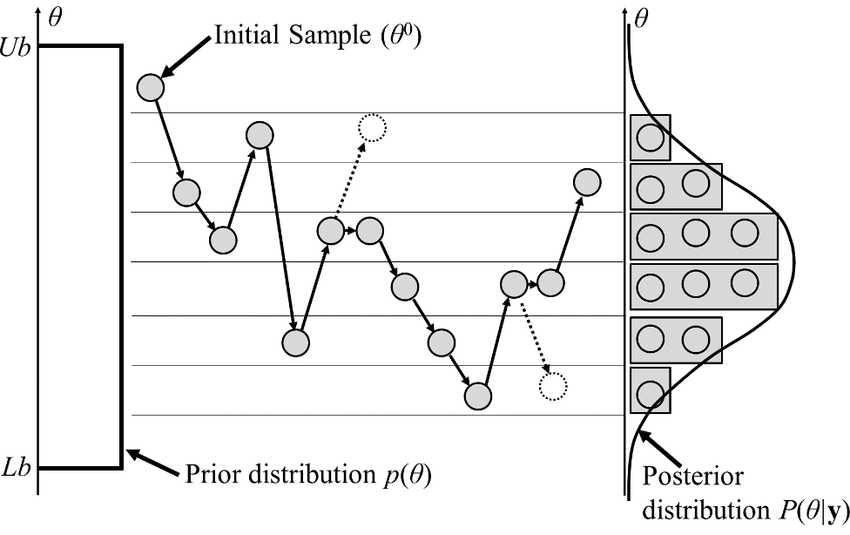
\includegraphics[width=.55\textwidth]{mh}
   \caption{Representation of the Metropolis-Hastings algorithm (taken from \citet{jaewook2015metamodel}). The discarded proposals are represented by dashed circles.}\label{fig:mh}
 \end{figure}

Figure~\ref{fig:mh} shows a schematic representation of the process. Note that \(f(x')/f(x_t)=\pi(x')/\pi(x_t)\) is a measure of how more likely is \(x'\) to be a sample from \(\pi\) than \(x_t\). This specific acceptance rate is also chosen so that the detailed balance equations of the chain are satisfied, i.e., \(\pi(x)P(x'|x)=\pi(x')P(x|x')\), where \(P(x|y)\) represents the transition probability from state \(x\) to state \(y\). These conditions essentially guarantee that \(\pi\) is the stationary distribution of the chain; see \citet{robert1999monte} for additional details. An immediate generalization consists on choosing a general (possibly non-symmetric) jump distribution \(g\), in which case the acceptance probability is rewritten as
\[
\alpha = \min\left\{1, \frac{f(x')g(x_t \mid x')}{f(x_t)g(x'\mid x_t)}\right\}.
\]

Although this algorithm performs well on a wide range of problems, it can be difficult to find a suitable jump distribution when the number of dimensions is high. If we know the conditional distribution of each variable on the rest of them, an alternative approach to sampling is \textit{Gibb's algorithm} \citep{geman1984stochastic}, which is a particular case of Metropolis-Hastings that considers separate samples for each dimension. Specifically, in each step we get unidimensional samples \textit{in turn} (e.g. via rejection sampling) of each variable conditional on the rest of them, using always the more up-to-date values available:

\[
\pi(x_l^{(i+1)} \mid x_{1}^{(i+1)}, \dots, x_{l-1}^{(i+1)}, x_{l+1}^{(i)}, \dots, x_L^{(i)}), \quad l=1,\dots,L.
\]

Lastly, there are several methods based on Metropolis-Hastings that are the subject of active research, both from a theoretical and computational standpoint. A good example are \textit{Hamiltonian Monte Carlo} methods \citep[e.g.][]{neal2011mcmc}, which are a family of algorithms that introduce gradient information to guide the proposals in the sample space. They are based on Hamiltonian dynamics, and in general they improve convergence speed due to a more intelligent choice of new points on the chain. With automatic differentiation being developed in the last few decades, these algorithms have become computationally feasible and have been widely adopted by the scientific community.

\subsection*{Affine-invariant ensemble sampler}

An interesting and often desirable property of sampling algorithms is that they be \textit{affine-invariant}, which means that they regard two distributions that differ in an affine transformation, say \(\pi(x)\) and \(\pi_{A, b}(Ax + b)\), as equally difficult to sample from. This is useful when one is working with very asymmetrical or skewed distributions, for an affine transformation can turn them into ones with simpler shapes.

Generally speaking, a MCMC algorithm can be described at time \(t+1\) as \(\Lambda(t+1)=R(\Lambda(t), \xi(t), \pi)\), where \(\Lambda(t)\) is the state of the chain at instant \(t\), \(\pi(x)\) is the objective distribution, and \(\xi(t)\) is a sequence of i.i.d. random variables that represent the random behavior of the chain. With this notation, the property of affine-invariant can be characterized as \citep{goodman2010ensemble}:
 \[
 R(A\lambda+b, \xi(t), \pi_{A,b}) = AR(\lambda, \xi(t), \pi) + b,
 \]
 for all \(A,b\) and \(\lambda\), and for almost all \(\xi(t)\). This means that if we fix a random generator and run the algorithm twice, one time using \(\pi\) and starting in \(\Lambda(0)\) and a second time using \(\pi_{A,b}\) with initial point \(\Gamma(0)=A\Lambda(0)+b\), then \(\Gamma(t)=A\Lambda(t)+b\) for all \(t\). In \citet{goodman2010ensemble} the authors consider an ensemble of samplers with the affine invariance property. Specifically, they work with a set \(\Lambda=(\Lambda_1, \dots, \Lambda_L)\) of \textit{walkers}, where \(\Lambda_l(t)\) represents an individual chain at time \(t\). At each iteration, an affine-invariant transformation is used to find the next point, which is constructed using the current values of the rest of the walkers (similar to Gibb's algorithm), namely the \textit{complementary ensemble}
 \[
  \Lambda_{-l}(t) = \{\Lambda_1(t+1), \dots, \Lambda_{l-1}(t+1), \Lambda_{l+1}(t), \dots, \Lambda_L(t)\}, \quad l=1,\dots, L.
  \]

To maintain the affine invariance and the joint distribution of the ensemble, the walkers are advanced one by one following a Metropolis-Hastings acceptance scheme. There are mainly two types of moves.

  \paragraph{Stretch move.} For each walker \(1\leq l \leq L\) another walker \(\Lambda_j \in \Lambda_{-l}(t)\) is chosen at random, and the proposal is constructed as
  \[
    \Lambda_l(t) \to \Gamma = \Lambda_j + Z(\Lambda_l(t) - \Lambda_j),
  \]
  where \(Z \stackrel{i.i.d.}{\sim} g(z)\) satisfying the symmetry condition \(g(z^{-1})=zg(z)\). In particular, the suggested density is
  \[
  g_a(z) \propto \begin{cases}
    \frac{1}{\sqrt{z}}, & \text{if } z \in [a^{-1}, a],\\
    0, & \text{otherwise.}
\end{cases}, \quad a > 1.
  \]
Supposing \(\R^p\) is the sample space, the corresponding acceptance probability (chosen so that the detailed balance equations are satisfied) is:
  \[
    \alpha = \min\left\{1, \ Z^{p-1}\frac{\pi(\Gamma)}{\pi(\Lambda_l(t))}\right\}.
  \]

  \paragraph{Walk move.} For each walker \(1\leq l \leq L\) a random subset \(S_l \subseteq \Lambda_{-l}(t)\) with \(|S_l| \geq 2\) is chosen, and the proposed move is
\[
\Lambda_l(t) \to \Gamma = \Lambda_l(t) + W,
\]
where \(W\) is a normal distribution with mean \(0\) and the same covariance as the sample covariance of all walkers in \(S_l\). The acceptance probability in this case is just the Metropolis ratio, i.e., \(\alpha=\min\{1, \pi(\Gamma)/\pi(\Lambda_l(t))\}\).\\

From a computational perspective, the Python library \textit{emcee}\footnote{\url{https://emcee.readthedocs.io/en/stable/}} \citep{foreman2013emcee} provides a parallel implementation of this algorithm. The idea is to divide the ensemble \(\Lambda\) into two equally-sized subsets \(\Lambda^{(0)}\) and \(\Lambda^{(1)}\), and then proceed on each iteration in the following alternate fashion:

\begin{enumerate}[1.]
  \item Update \textit{all} walkers in \(\Lambda^{(0)}\) through one of the available moves explained above, using \(\Lambda^{(1)}\) as the complementary ensemble.
  \item Use the new values in \(\Lambda^{(0)}\) to update \(\Lambda^{(1)}\).
\end{enumerate}

In this way the detailed balance equations are still satisfied, and each of the steps can benefit from the computing power of an arbitrary number of processors (up to \(L/2\)).
